We compare the performance of \sys against the state-of-the-art intermittent execution approach---Chain~\cite{chain}.

The applications that were used in the evaluation are given in Table~\ref{table:benchmark_list}.

\begin{table}
	\begin{tabular}{|c|c|c|}
		\hline
		Name & SLOC (\sys) & SLOC (Chain~\cite{chain})\\
		\hline\hline
		Temperature sensing & 388 & 721 \\ %53\%
		Cuckoo & 483 & 762 \\ %63\%
		RSA & 887 & 1233 \\ %71\%
		DFT & --- & --- \\ %Two resolutions: 4 and 8 Bytes
		Huffman & --- & --- \\ %Data decompression size: 100 bytes
		Selection sort & --- & --- \\
		\hline
	\end{tabular}
\caption{List of benchmarks used in \sys evaluation.}
\label{table:benchmark_list}
\end{table}

\subsection{Continuous Power Supply}
\label{sec:results_continuous_power}

\begin{figure}
	\centering
	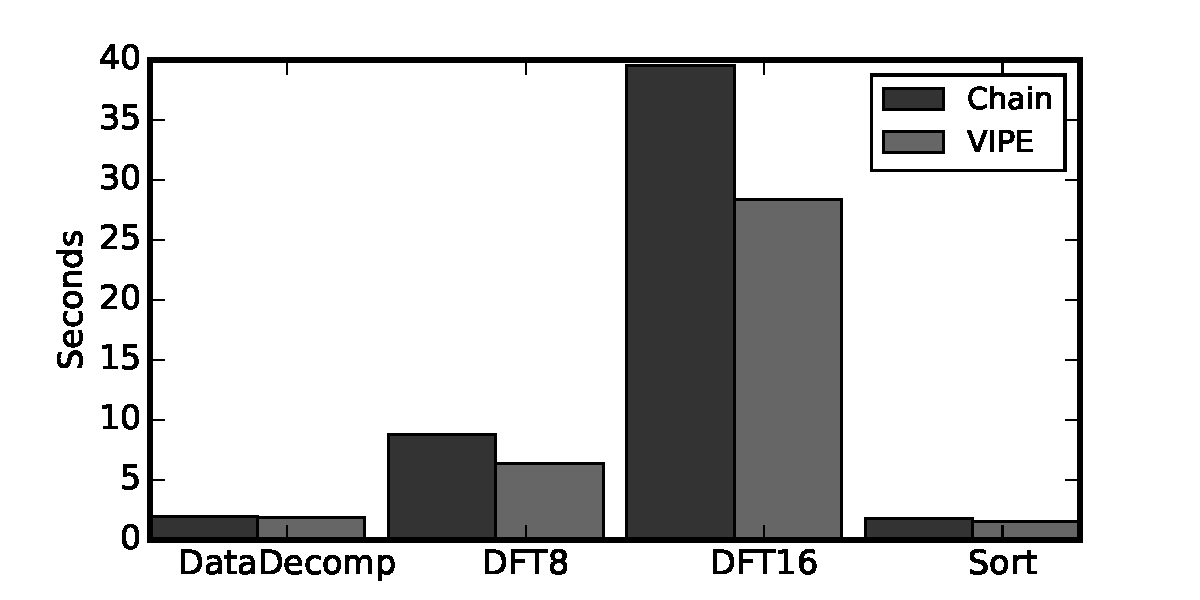
\includegraphics[width=\columnwidth]{figures/chain_vipe}
	\caption{Time to complete for a set of testing applications (refer to Table~\cite{table:benchmark_list}) using \sys versus Chain.}
	\label{fig:IPOSPerformance}
\end{figure}

Fig.~\ref{fig:IPOSPerformance} shows that \sys requires a shorter execution time to execute an application under the modular execution model. The size of the virtual task that \sys uses is one real task, i.e. no task coalescing is applied.

%Set of experiments

%- Compiler result: taskifying completion time, correctness, 
%- Task coalescing experiment: with WISP at 3 distances and with fixed power, for all apps, compared against chain, show amount of task merged, time to completion/inter-operation time, overhead (in terms of what?), energy consumed
%- Battery-less microphone: with \sys and without \sys, compared against Chain, 
%- Paging/memory experiment: ?

\subsection{Intermittent Power Supply}
\label{sec:intermittent_continuous_power}